\documentclass[12pt]{article}
\usepackage[margin=1in]{geometry}
\usepackage{setspace}
\onehalfspacing

% Start of preamble
%==========================================================================================%
% Required to support mathematical unicode
\usepackage[warnunknown, fasterrors, mathletters]{ucs}
\usepackage[utf8x]{inputenc}

\usepackage[dvipsnames,table,xcdraw]{xcolor}

% Standard mathematical typesetting packages
\usepackage{amsmath,amssymb,amscd,amsthm,amsxtra, pxfonts}
\usepackage{mathtools,mathrsfs,dsfont,xparse}

% Symbol and utility packages
\usepackage{cancel, textcomp}
\usepackage[mathscr]{euscript}
\usepackage[nointegrals]{wasysym}
\usepackage{apacite}

% Extras
\usepackage{physics}  
\usepackage{tikz-cd} 
\usepackage{microtype}
\usepackage{enumitem}
\usepackage{titling}
\usepackage{graphicx}

% Fancy theorems due to @intuitively on discord
\usepackage{mdframed}
\newmdtheoremenv[
backgroundcolor=NavyBlue!30,
linewidth=2pt,
linecolor=NavyBlue,
topline=false,
bottomline=false,
rightline=false,
innertopmargin=10pt,
innerbottommargin=10pt,
innerrightmargin=10pt,
innerleftmargin=10pt,
skipabove=\baselineskip,
skipbelow=\baselineskip
]{mytheorem}{Theorem}

\newenvironment{theorem}{\begin{mytheorem}}{\end{mytheorem}}

\newtheorem{corollary}{Corollary}
\newtheorem{lemma}{Lemma}

\newtheoremstyle{definitionstyle}
{\topsep}%
{\topsep}%
{}%
{}%
{\bfseries}%
{.}%
{.5em}%
{}%
\theoremstyle{definitionstyle}
\newmdtheoremenv[
backgroundcolor=Violet!30,
linewidth=2pt,
linecolor=Violet,
topline=false,
bottomline=false,
rightline=false,
innertopmargin=10pt,
innerbottommargin=10pt,
innerrightmargin=10pt,
innerleftmargin=10pt,
skipabove=\baselineskip,
skipbelow=\baselineskip,
]{mydef}{Definition}
\newenvironment{definition}{\begin{mydef}}{\end{mydef}}

\newtheorem*{remark}{Remark}

\newtheorem*{example}{Example}

% Common shortcuts
\def\mbb#1{\mathbb{#1}}
\def\mfk#1{\mathfrak{#1}}

\def\bN{\mbb{N}}
\def \C{\mbb{C}}
\def \R{\mbb{R}}
\def\bQ{\mbb{Q}}
\def\bZ{\mbb{Z}}
\def \cph{\varphi}
\renewcommand{\th}{\theta}
\def \ve{\varepsilon}
\newcommand{\mg}[1]{\| #1 \|}

% Often helpful macros
\newcommand{\floor}[1]{\left\lfloor#1\right\rfloor}
\newcommand{\ceil}[1]{\left\lceil#1\right\rceil}
\renewcommand{\qed}{\hfill\qedsymbol}
\renewcommand{\P}{\mathbb P\qty}
\newcommand{\E}{\mathbb{E}\qty}
\newcommand{\Cov}{\mathrm{Cov}\qty}
\newcommand{\Var}{\mathrm{Var}\qty}

% Sets
\usepackage{braket}

\graphicspath{{/}}
\usepackage{float}

\newcommand{\SET}[1]{\Set{\mskip-\medmuskip #1 \mskip-\medmuskip}}

% End of preamble
%==========================================================================================%

% Start of commands specific to this file
%==========================================================================================%

\usepackage{booktabs}

%==========================================================================================%
% End of commands specific to this file

\title{CSE 422 HW1}
\date{\today}
\author{Rohan Mukherjee}

\begin{document}
    \maketitle
    \begin{enumerate}[leftmargin=\labelsep]
        \item 
        \begin{enumerate}[label=(\alph*)]
            \item I have written it.

            \item The pro of the first strategy is that it is the computationally fastest of all of them. It needs to make only one random call and has no if statements in it. However, all the other methods are theoretically better than this method, since they sample a uniform bin, but compare it with at least 1 other bin and puts the ball in the bin with fewer balls. 
            
            The second method and fourth method are similar, except I believe the second method is more expensive. But it also would theoretically perform the best: see the last part. The next method saves by not having to make another random call.

            This third method should just be a generalization of the second method, but with a third random call and now a more if statements since it has to find which bin has the fewest elements. So this is the best method, but it would also be the most expensive to implement or do at large scale.

            Here is a plot:
            \begin{figure}[H]
                \centering
                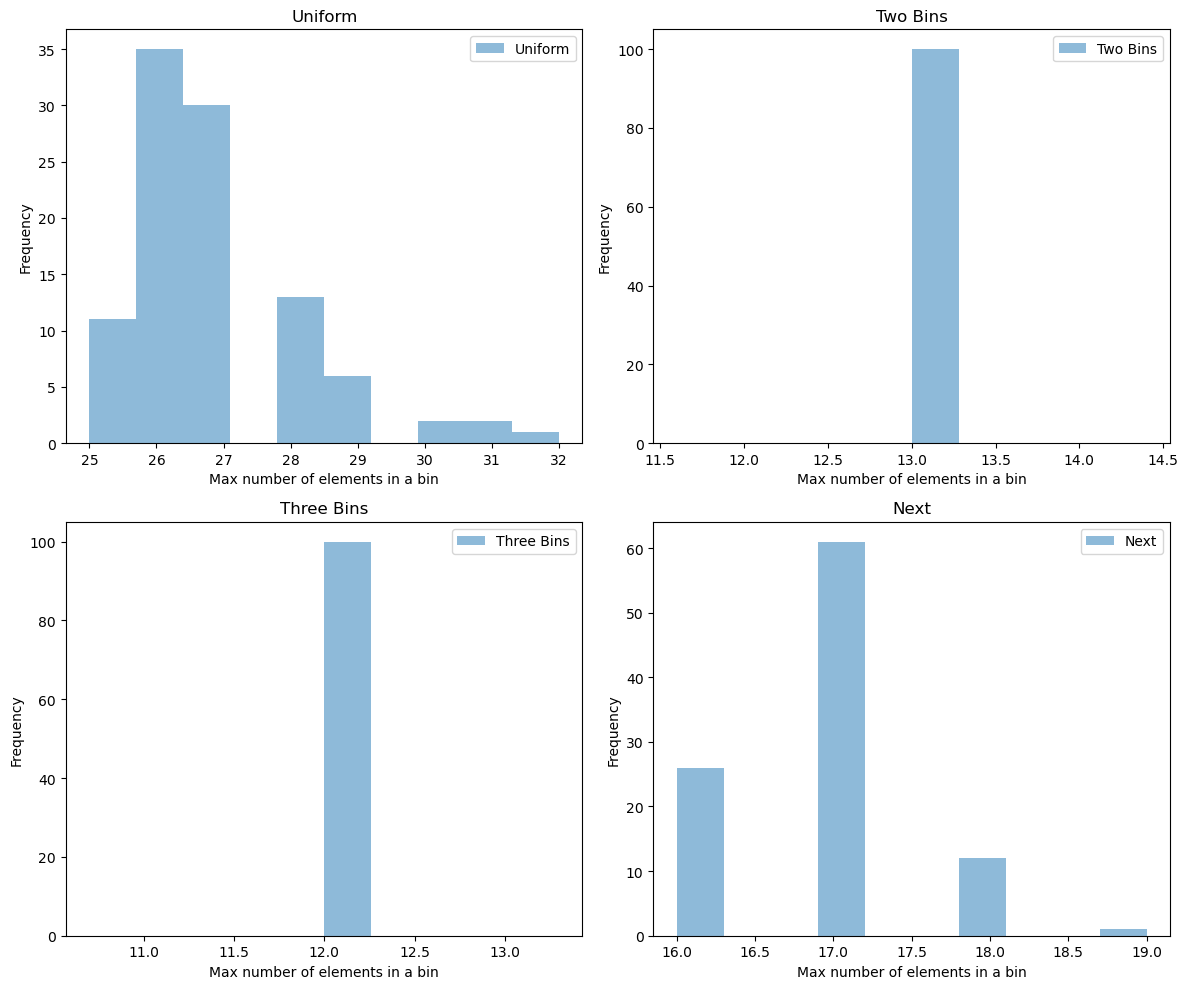
\includegraphics[width=0.8\textwidth]{histogram.png}
                \caption{Histogram of the results}
                \label{fig:histogram}
            \end{figure}


            \item To model consistent hashing as a balls-into-bins problem, we can think of the servers as the bins and the keys as the balls. What we are doing right now is hashing the bins and putting them on a circle, and hashing the keys, and putting them on a circle too, and putting all the keys that fall in the clockwise arc connecting two bins into the first bin. Right now, without having servers go out, this is equivalent to just uniformly sampling a bin to put the key in, assuming the hashing function is "sufficiently random". Since in expectation all the arcs have the same length and the hash function should hash to a random point on the circle uniformly.

            However, the previous homework questions showed us that uniformly sampling is not the best option. From the histogram (and from part e), it seems like the best option is where we uniformly sample 3 bins  and then put the ball in the one that has the smallest number of balls. For the 3 bins sampled method, to make this back into the consistent hashing problem, we could have multiple hash functions that hash the key multiple times, which is like putting the key into multiple random arcs, and putting the ball in the arc (server) with fewest balls.

            This idea can be extended to the others as well. The 2-bin version is just a simplification of this. The uniform is what we are doing right now, and the next sampling method is just hash the key once, and check the arc it falls in and the arc that is after it clockwise.

            \item I do not think that the first strategy, just uniformly sampling, can be represented in this graph way. This is because there is no consideration of which bin has fewer balls, since it doesn't care about that and just does it randomly. Unless we could somehow use an empty graph with n points that are not connected to each other, but this doesn't have any edges, so I don't think so.

            On the other hand, the second strategy can be represnted in this way. Consider the complete graph $K_n$. Then picking a random edge will just uniformly pick two bins, and we will put it in the one with fewer balls. This is precisely the second strategy.

            The third strategy, which compares 3 bins, is not possible, because we would need to consider 3 bins, not two, but there is only 2 vertices for each edge.

            The last strategy, which I call the ``next'' strategy, is easier to represent on a graph. This is just the cycle graph $C_n$. When we select an edge $(i, i+1)$, it compares $i$ to $i+1$ and puts it in the bin with fewer balls. 

            \item I believe that some graphs do better than others based on how "connected" they are. For example, in the worst possible case where we only have 1 edge connecting two vertices, we know that the max load will be huge, since all the load goes on those two vertices. On the other hand, for cyclic graph like the next method does, we know that it can only compare bins that are 1 away from each other. Intuitively, it seems that if we had a high load in a bin, then the nearby bins would also have high load. But in this case we can only look at one other bin once we have drawn the high load bin, which would mean that these bins combined must have high load. The opposite of this strategy is the most connected graph $K_n$, where once we have picked a bin, we can with equal probability see any other bin, which gives us a lot more options to offload the weight than just the next bin. 

            \item From this connectedness idea, I looked up what is the best 3-regular connected graph, and it seems like expander graphs do the job well. So I would pick a 3-regular expander graph. 
        \end{enumerate}

        \item
        \begin{enumerate}[label=(\alph*)]
            \item It has been done.
            \item The total number of elements in this dataset is $\sum_{i=1}^n i^2 + (n^2-n) = \frac{2n^3+9n^2-5n}{6}$. So we are looking for elements $x$ with the frequency of $x$ being $\geq \frac{2n^3+9n^2-5n}{600}$.

            \item This is the table I get:
            \begin{table}[h!]
                \centering
                \begin{tabular}{lrr}
                \toprule
                Category & Average Frequency of 100 & Average Number of Heavy Hitters \\
                \midrule
                Heavy First & 10082.00 & 43.30 \\
                Heavy Last  & 10082.00 & 43.00 \\
                Random      & 10082.00 & 43.30 \\
                \bottomrule
                \end{tabular}
                \caption{Unoptimized Results}
            \end{table}

            As you can see, they all the get exact same frequency of 100s, and they have a very similar number of heavy hitters, up to variance of 0.3. There is absolutely no variance in the frequency of 100s, since the hash function is the same for the 3 different datasets. Once you have fixed the hash function, for any permutation of the dataset, you will hash the keys in a different order to the same place, which leads to the same counts. 

            On the other hand, variance in the heavy hitters can be explained by collisions. Suppose that for some number in the dataset, say $x$ that is more than 1\% of the dataset, we had another number that gets hashed to the same place. If this happens before we have counted all the $x$'s, such as in the heavy last, this won't matter because it won't occupy the same space as a heavy hitter until after we have counted all of the low-frequency ones. However, when the order is changed, such as in heavy first/random, we could see a low-frequency collision after $x$ takes more than 1\% of the dataset, which would add to the number of heavy hitters.

            \item We prove this statement by induction on the frequency of a fixed element $x$ in the dataset. For the first time, when we hash $x$ and are supposed to put it in the counts matrix, we only update the subset of counters for which the count is minimal. Either all counts are 0, in which case they will all be updated, or some are 0 and others aren't, in which case after updating those that are 0, all the counters corresponding to the hash of $x$ will be greater than or equal to 1. 

            Now suppose that the we have counted the $n-1$th frequency of $x$, and all the counters are $\geq n-1$. On the $n$th encounter of $x$, either there are some counters that are $n-1$ or not. When there are not, all counters are already bigger than $n$ and we are done. On the other hand, since $n-1$ is the minimum the counter can be, we will update all the counters that are $n-1$ to $n$. Then in this case all the counters coresponding to $x$ are $\geq n$, and we are again done.

            \newpage
            \item This is wht I get for the conservative updates:
            \begin{table}[h!]
                \centering
                \begin{tabular}{lrr}
                \toprule
                Category & Average Frequency of 100 & Average Number of Heavy Hitters \\
                \midrule
                Heavy First & 10000.00 & 43.20 \\
                Heavy Last  & 10033.80 & 43.00 \\
                Random      & 10000.00 & 43.00 \\
                \bottomrule
                \end{tabular}
                \caption{Optimized Results}
            \end{table}

            As before, the average number of heavy hitters is expected to have some variance since low-frequency collisions can happen and will update the set of heavy hitters with fake ones. However, the aaverage frequency of 100 is now different too. This is because the conservative update optimization, which updates only the minimum counters, adds an order dependence to the counts. For example, if we process everything before the number 100, then probably all the counters associated with the hash of 100 will already have some counts, and so when we add the $100^2$ 100s, the minimum count will be higher than if we had processed the 100s first. On the other hand, if we process all the $100^2$ 100s first, then all the counters associated with 100 will go straight to 10,000. When low-frequency collisions happen, the 10,000 will ALWAYS be the highest count among them, and hence will not be updated. This explains why the average frequency count for 100 is higher in heavy last, and why it is low in heavy first. For random, you are certainly likely to see lots of the 10,000 100s before seeing any collisions with 100, so the same logic applies but at a lower scale than with heavy last.
        \end{enumerate}
    \end{enumerate}
\end{document}